\chapter{Attention-based architectures}


\begin{description}
    \item[Sequence-to-sequence (seq2seq) model] \marginnote{Sequence-to-sequence (seq2seq) model}
        Encoder-decoder architecture where:
        \begin{descriptionlist}
            \item[Encoder] 
                Processes the whole input sequence and outputs a representation of it.

            \item[Decoder] 
                Processes the output of the encoder and produces the output sequence.
        \end{descriptionlist}

        \begin{remark}
            Training is usually done using teacher forcing and averaging the loss of each output distribution.
        \end{remark}

        \begin{figure}[H]
            \centering
            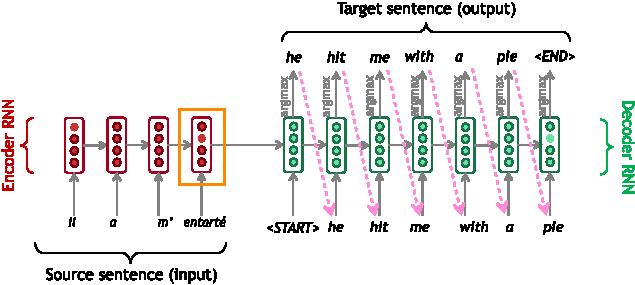
\includegraphics[width=0.7\linewidth]{./img/_seq2seq.pdf}
            \caption{Example of seq2seq network with RNNs}
        \end{figure}
\end{description}



\section{Encoder-decoder RNN with attention}

\begin{description}
    \item[Seq2seq RNN with attention] \marginnote{Seq2seq RNN with attention}
        Architecture where the decoder can interact with each token processed by the encoder to determine dot-product attention scores (i.e., based on vector similarity).

        The overall flow is the following:
        \begin{enumerate}
            \item The encoder computes its hidden states $\vec{h}^{(1)}, \dots, \vec{h}^{(N)} \in \mathbb{R}^{h}$.
            \item The decoder processes the input tokens one at the time beginning with a \texttt{<start>} token. Its hidden state is initialized with $\vec{h}^{(N)}$. Consider the token at position $t$, the output is determined as follows:
            \begin{enumerate}
                \item The decoder outputs the hidden state $\vec{s}^{(t)}$.
                \item Attention scores $\vec{e}^{(t)}$ are determined as the dot product between $\vec{s}^{(t)}$ and $\vec{h}^{(i)}$:
                \[ 
                    \vec{e}^{(t)} = 
                        \begin{bmatrix}
                            \vec{s}^{(t)} \cdot \vec{h}^{(1)} & 
                            \cdots &
                            \vec{s}^{(t)} \cdot \vec{h}^{(N)} 
                        \end{bmatrix} \in \mathbb{R}^{N} 
                \]
                $\vec{e}^{(t)}$ is used to determine the attention distribution $\vec{\alpha}^{(t)}$ that is required to obtain the attention output $\vec{a}^{(t)}$ as the weighted sum of the encoder hidden states:
                \[
                    \begin{gathered}
                        \mathbb{R}^{N} \ni \vec{\alpha}^{(t)} = \texttt{softmax}(\vec{e}^{(t)}) \\
                        \mathbb{R}^{h} \ni \vec{a}^{t} = \sum_{i=1}^{N} \vec{\alpha}^{(t)}_i \vec{h}^{(i)}
                    \end{gathered}
                \]
                \item The overall representation of the $t$-th token is the concatenation of the attention and decoder output:
                \[ \begin{bmatrix} \vec{a}^{(t)} \mid \vec{s}^{(t)} \end{bmatrix} \in \mathbb{R}^{2h} \]
            \end{enumerate}
        \end{enumerate}

        \begin{figure}[H]
            \centering
            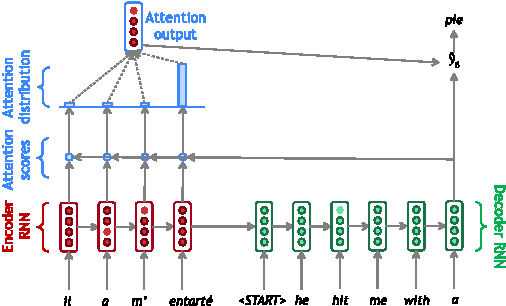
\includegraphics[width=0.6\linewidth]{./img/_rnn_attention.pdf}
        \end{figure}
\end{description}



\section{Convolutional neural networks for NLP}

\begin{description}
    \item[1D convolution (NLP)] \marginnote{1D convolution}
        Apply a kernel on a sequence of tokens within a window. A kernel of size $k$ with $d$-dimensional token embeddings is represented by a $k \times d$ weight matrix.

        \begin{remark}
            As in computer vision, multiple kernels can be stacked to increase the depth of the representation. Padding, stride, and dilation can also be used to change the receptive field. Pooling is also performed before passing to fully-connected layers.
        \end{remark}

        \begin{figure}[H]
            \centering
            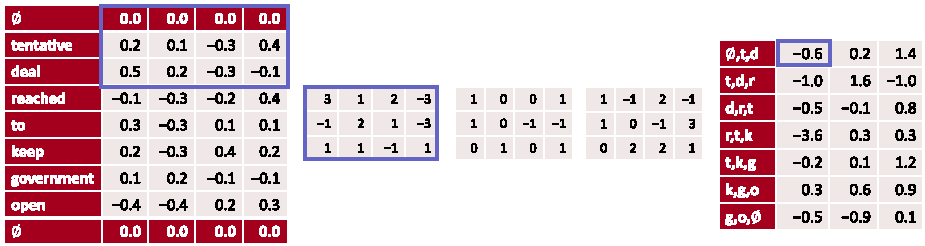
\includegraphics[width=0.8\linewidth]{./img/_1d_convolution.pdf}
            \caption{Example of three 1D convolutions with padding $1$}
        \end{figure}
\end{description}

\begin{remark}
    Convolutions are easy to parallelize.
\end{remark}

\begin{example}[CNN for sentence classification]
    A possible multichannel CNN architecture for sentence classification works as follows:
    \begin{itemize}
        \item The input sequence is encoded by stacking both static and learned embeddings (of the same dimensionality).
        \item Convolutions are applied to each channel. They can work with different widths.
        \item Pooling is used to flatten the activations and avoid shape mismatch before passing through fully-connected layers.
    \end{itemize}

    \begin{figure}[H]
        \centering
        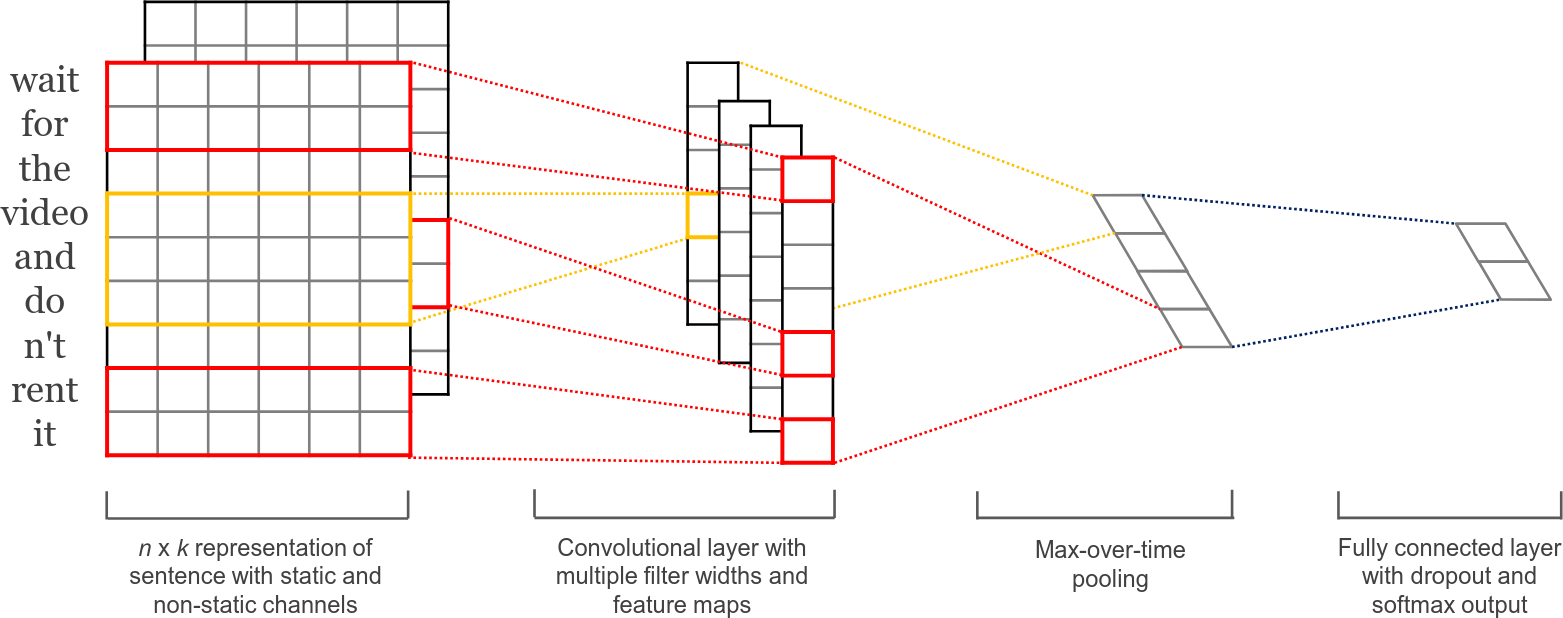
\includegraphics[width=0.7\linewidth]{./img/cnn_sentence_classification.png}
    \end{figure}
\end{example}

\begin{example}[Character-aware neural LM]
    \phantom{}\\
    \begin{minipage}{0.6\linewidth}
        RNN-LM that works on the character level:
        \begin{itemize}
            \item Given a token, each character is embedded and concatenated.
            \item Convolutions are used to refine the representation.
            \item Pooling is used before passing the representation to the RNN.
        \end{itemize}
    \end{minipage}
    \begin{minipage}{0.35\linewidth}
        \centering
        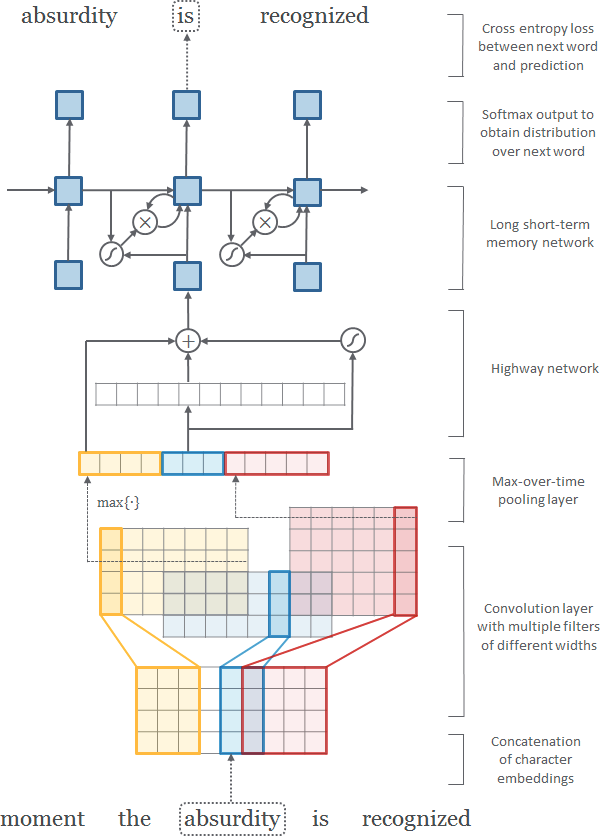
\includegraphics[width=0.95\linewidth]{./img/char_aware_rnn_cnn.png}
    \end{minipage}


\end{example}



\section{Transformer decoder (for language modelling)}


\subsection{Self-attention}

\begin{description}
    \item[Self-attention] \marginnote{Self-attention}
        Component that allows to compute the representation of a token considering the other ones in the input sequence. 

        Given an input embedding $\vec{x}_i \in \mathbb{R}^{1 \times d_\text{model}}$, self-attention relies on the following values:
        \begin{descriptionlist}
            \item[Queries] \marginnote{Queries}
                Used as the reference point for attention:
                \[ \mathbb{R}^{1 \times d_k} \ni \vec{q}_i = \vec{x}_i \matr{W}_Q \]
            \item[Keys] \marginnote{Keys}
                Used as values to compare against the query:
                \[ \mathbb{R}^{1 \times d_k} \ni \vec{k}_i = \vec{x}_i \matr{W}_K \]
                \item[Values] \marginnote{Values}
                Used to determine the output:
                \[ \mathbb{R}^{1 \times d_v} \ni \vec{v}_i = \vec{x}_i \matr{W}_V \]
            \end{descriptionlist}
        where $\matr{W}_Q \in \mathbb{R}^{d_\text{model} \times d_k}$, $\matr{W}_K \in \mathbb{R}^{d_\text{model} \times d_k}$, and $\matr{W}_V \in \mathbb{R}^{d_\text{model} \times d_v}$ are parameters.

        Then, the attention weights $\alpha_{i,j}$ between two embeddings $\vec{x}_i$ and $\vec{x}_j$ are computed as:
        \[
            \begin{gathered}
                \texttt{score}(\vec{x}_i, \vec{x}_j) = \frac{\vec{q}_i \vec{k}_j}{\sqrt{d_k}} \\
                \alpha_{i,j} = \texttt{softmax}_j\left( \left[\texttt{score}(\vec{x}_i, \vec{x}_1), \dots, \texttt{score}(\vec{x}_i, \vec{x}_T)\right] \right) \\
            \end{gathered}
        \]
        The output $\vec{a}_i \in \mathbb{R}^{1 \times d_v}$ is a weighted sum of the values of each token:
        \[ \vec{a}_i = \sum_{t} \alpha_{i,t} \vec{v}_t \]

        To maintain the input dimension, a final projection $\matr{W}_O \in \mathbb{R}^{d_v \times d_\text{model}}$ is applied.

        \begin{figure}[H]
            \centering
            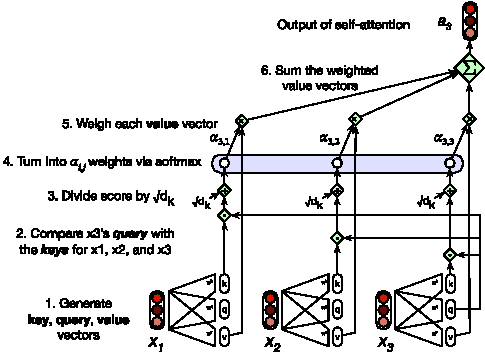
\includegraphics[width=0.6\linewidth]{./img/_self_attention.pdf}
        \end{figure}


    \item[Causal attention] \marginnote{Causal attention}
        Self-attention mechanism where only past tokens can be used to determine the representation of a token at a specific position. It is computed by modifying the standard self-attention as follows:
        \[
            \begin{gathered}
                \forall j \leq i: \texttt{score}(\vec{x}_i, \vec{x}_j) = \frac{\vec{q}_i \vec{k}_j}{\sqrt{d_k}} \qquad
                \forall j > i: \texttt{score}(\vec{x}_i, \vec{x}_j) = -\infty \\
                \alpha_{i,j} = \texttt{softmax}_j\left( \left[\texttt{score}(\vec{x}_i, \vec{x}_1), \dots, \texttt{score}(\vec{x}_i, \vec{x}_T)\right] \right) \\
                \vec{a}_i = \sum_{t: t \leq i} \alpha_{i,t} \vec{v}_t
            \end{gathered}
        \]

        \begin{figure}[H]
            \centering
            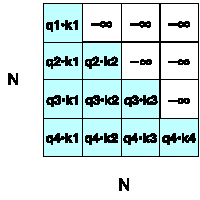
\includegraphics[width=0.2\linewidth]{./img/_masked_attention.pdf}
            \caption{Score matrix with causal attention}
        \end{figure}
\end{description}


\subsection{Embeddings}

\begin{description}
    \item[Input embedding] \marginnote{Input embedding}
        The input is tokenized using standard tokenizers (e.g., BPE, SentencePiece, \dots). Each token is then encoded using a learned embedding matrix.

        \begin{figure}[H]
            \centering
            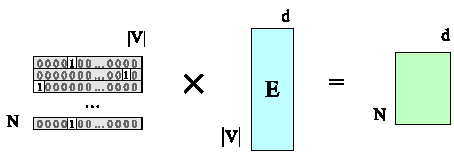
\includegraphics[width=0.45\linewidth]{./img/_transformer_embedding.pdf}
        \end{figure}

    \item[Positional encoding] \marginnote{Positional encoding}
        Learned position embeddings to encode positional information are added to the input token embeddings.

        \begin{remark}
            Without positional encoding, transformers are invariant to permutations.
        \end{remark}

        \begin{figure}[H]
            \centering
            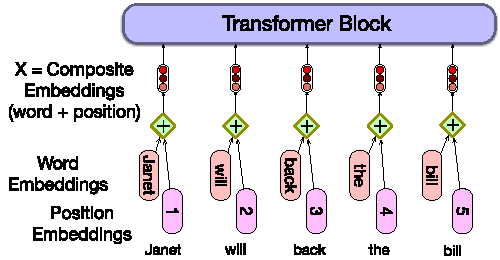
\includegraphics[width=0.45\linewidth]{./img/_positional_encoding.pdf}
        \end{figure}
\end{description}


\subsection{Transformer block}

\begin{description}
    \item[Transformer block] \marginnote{Transformer block}
        Module with the same input and output dimensionality (i.e., allows stacking multiple blocks) composed of:
        \begin{descriptionlist}
            \item[Multi-head attention] \marginnote{Multi-head attention}
                Uses $h$ different self-attention blocks with different queries, keys, and values. Value vectors are of size $\frac{d_v}{h}$. The final projection $W_O$ is applied on the concatenation of the outputs of each head.

                \begin{figure}[H]
                    \centering
                    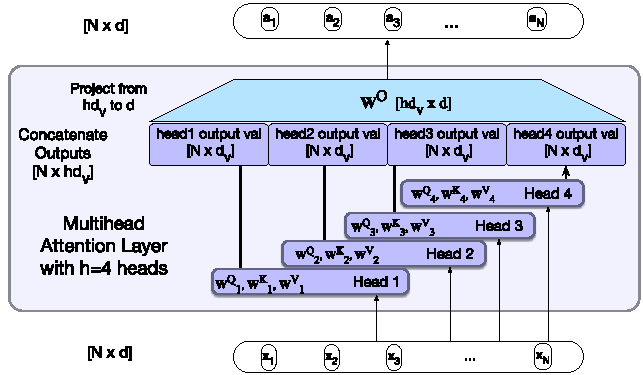
\includegraphics[width=0.6\linewidth]{./img/_multi_head_attention.pdf}
                \end{figure}

            \item[Feedforward layer]
                Fully-connected 2-layer network applied at each position of the attention output:
                \[ \texttt{FFN}(\vec{x}_i) = \texttt{ReLU}(\vec{x}_i\matr{W}_1 + \vec{b}_1)\matr{W}_2 + \vec{b}_2 \]
                Where the hidden dimension $d_\text{ff}$ is usually larger than $d_\text{model}$.

            \item[Normalization layer]
                Applies layer normalization (i.e., normalize each sequence of the batch independently) to help training stability.

            \item[Residual connection]
                Helps to propagate information during training.

                \begin{remark}[Residual stream]
                    An interpretation of residual connections is that of residual stream where the input token is enhanced by the output of multi-head attention and the feedforward network.

                    \begin{figure}[H]
                        \centering
                        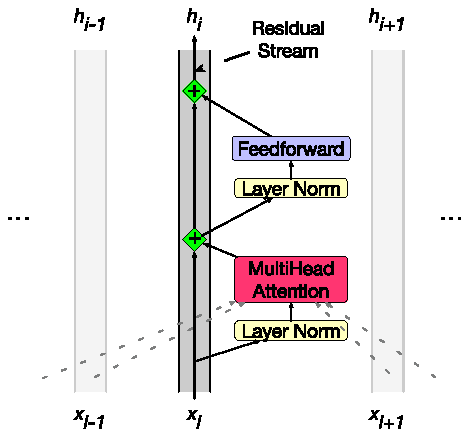
\includegraphics[width=0.38\linewidth]{./img/_residual_stream.pdf}
                    \end{figure}
                \end{remark}
        \end{descriptionlist}

        \begin{figure}[H]
            \centering
            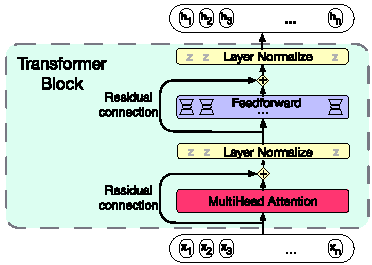
\includegraphics[width=0.4\linewidth]{./img/_attention_block.pdf}
            \caption{Overall attention block}
        \end{figure}

    \item[Language modeling head] \marginnote{Language modeling head}
        Takes as input the output corresponding to a token of the transformer blocks stack and outputs a distribution over the vocabulary.

        \begin{figure}[H]
            \centering
            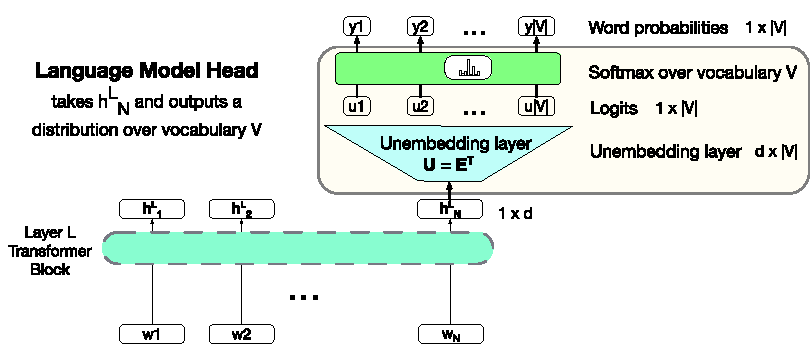
\includegraphics[width=0.6\linewidth]{./img/_lm_head.pdf}
        \end{figure}
\end{description}